%\documentclass[conference]{IEEEtran}
%\documentclass[journal,onecolumn,draftclsnofoot,]{IEEEtran}
\documentclass[11pt]{article}
%\documentclass[conference]{IEEEtran}
%\documentclass{acm_proc_article-sp}
%%%% ADDED -- PPD --- START
\usepackage{graphicx}
\usepackage{float}
\usepackage{bbding}
\usepackage{enumerate}
\usepackage{fancyvrb}
\usepackage{color,soul}
\usepackage{graphicx}
\usepackage{float}
\usepackage{bbding}
\usepackage{enumerate}
\usepackage{color,soul}
\usepackage{graphicx}
\usepackage{float}
\usepackage{bbding}
\usepackage{amsmath}
\usepackage{xcolor}
%\usepackage{hyperref}
\usepackage{colortbl}
\usepackage{fancybox}
\usepackage{amssymb}
\usepackage{pdfpages}
\usepackage{tikz}
\usepackage{array}
\usepackage{multirow}
%\usepackage{subcaption}
\usepackage{capt-of}
\usepackage{color,soul}
\usetikzlibrary{fit,shapes.geometric}
\usepackage{latexsym}
\usepackage{hyperref}

%\usepackage[a4paper, lmargin=0.8in, rmargin=0.8in, tmargin=0.6in, bmargin=0.6in]{geometry}
\renewcommand{\thesection}{\Roman{section}} 
\usepackage[lmargin=1in, rmargin=1in, tmargin=1in, bmargin=1in]{geometry}

%\usepackage{enumitem}
%\usepackage[inline]{enumerate}
%\usepackage[inline]{enumitem}
%%%% ADDED -- PPD --- END
\begin{document}
\title{Applications of Image Processing in Computer Science}

\date{}
\maketitle
\thispagestyle{empty}

{\centering \textit {\large White Paper}\par}

\vspace{0.5cm}
{\centering \textit{\large Image Processing CS 40019}\par}
%
%\author{	Name:\\
%	Roll No: \\
%	Department: \\
%	Date: }
%	partha.p.das@gmail.com	}
%\date{}

	%\maketitle
\vspace{5.5cm}

{\centering \large{\textbf{Name:} Nishant Baranwal Somy}\par}

{\centering \large{\textbf{Roll No:} 15CS30044}\par}

\vspace{2.0cm}

\begin{figure}[h]
	\centering
	
\includegraphics[height=3cm,width=3cm]{IIT_Logo.png}
\end{figure}


\begin{center}
	{   
	    \textbf{Date:} 5$^{th}$ September 2018 \\
		\textbf{Department:} Computer Science and Engineering \\
		\textbf{Indian Institute of Technology, Kharagpur,}\\
		\textbf {WB 721302, India}\\
	}
\end{center}
\newpage
\tableofcontents

\newpage

\begin{center}
\section*{Abstract}
({\em Within 100 words)} 

Image processing in computer science is the use of computer algorithms to perform image processing on digital images. Its a very broad field and involves several tasks such as Classification, Feature extraction, Multi-scale signal analysis, etc. In this work, we try to explore three important applications which use image processing at its core which are estimating layout of a room using its 2-D image, enhancing photos clicked from low-end cameras, and 3-D reconstruction of a soccer game using its monocular video only. Later, we also try to suggest an idea for a new application using image processing.

\end{center}
\newpage
{\bf {\em Instructions}}:
A list of domain areas are given in:
 
\begin{center}
\href{https://drive.google.com/open?id=1AxEDpTxQRyBxRbU\_F9WZughFvBrF609W}
{https://drive.google.com/open?id=1AxEDpTxQRyBxRbU\_F9WZughFvBrF609W}
\end{center}

Kindly choose one domain area that is closest to your background. Mention your choice in the first section of the white paper and include it in the title. The rest of the sections in the white paper will be in the context of the domain area as chosen.

\newpage
\section{Domain Area}
({\em Within 50 words})\\

I have chosen Computer Science as my field as it is a very broad field and encompasses a lot of other fields including Image Processing. Not only that, Image Processing together with other subfields of computer science like Machine Learning, Computer Vision, Virtual Reality solve numerous wonderful applications in the real world.

\section{Introduction}
({\em Within 200 words}) \\

Image Processing finds numerous applications in computer science. It is used in Computer Graphics, Virtual Reality, Medical Imaging, Computer Vision, Robotics and the list goes on and on. It also has its hold on multitude of levels of applications. From microsensors in mobile cameras which does very fast on-device processing of images on hardware level to Object detection which does processing on higher level. Image processing is involved in multitude of tasks which we do on a daily basis. Whether we are clicking pictures, editing them, analysing them or transforming them. Some of these wonderful applications are identifying flood hit areas from satellite images, detecting number of cars breaking traffic rules using traffic footage, identifying thieves using gait and face recognition using security footage, etc. Image processing is a very fundamental field in computer science and its important to learn it carefully as it far-reaching applications. In this paper, we try to explore three extraordinary applications of image processing in real-world problems. We will also try to suggest a new application in the field and hope that its feasible using Image Processing.

\section{Applications}
List 3 applications and elaborate each according to the following template.

\subsection{Application 1: Construction of 3-D layout of rooms}


\subsubsection{Introduction} 
({\em Within 100 words}) \\

Estimating the 3-D layout of a room from one image is an important goal in fields like Robotics and Virtual/Augmented Reality. Some of these applications include indoor navigation, scene rendering, scene reconstruction, etc. The objective is to specify the positions, orientations, and heights of the walls, relative to the camera center given a perspective or panoramic image of a room. The layout can be represented as a set of projected corner positions or boundaries, or as a 3D mesh. Previous works have tried to solve a special case of this problem that is estimating the layout of L-shaped rooms that conform to manhattan layouts and in some cases only cuboidal manhattan rooms. In this study, we will looking at the approach used by state-of-the-art LayoutNet which generalises to non-cuboidal manhattan rooms as well.

%\subsubsection{Motivation and Usage} ({\em Within 50 words)} 
\subsubsection{Sensors, Type \& Band of imaging}
({\em Within 50 words}) \\

The input to the algorithm is a monocular perspective or panoramic image of a manhattan room.

\subsubsection{Algorithms / Processing} 
({\em Within 300 words})\\

\begin{enumerate}
    \item {\em \textbf{Panoramic Image Alignment}}: Given the input as a panorama that covers a 360◦ horizontal
field of view, we first align the image by estimating
the floor plane direction under spherical projection, rotate
the scene, and reproject it to the 2D equirectangular
projection. After this, it selects
long line segments using the Line Segment Detector
(LSD) in each overlapped perspective view, then vote
for three mutually orthogonal vanishing directions using the
Hough Transform. 
    
    \item {\em \textbf{Corner and Boundary prediction using CNN}}: An overview of the LayoutNet network is illustrated in
Fig. 2. The network follows an encoder-decoder strategy.
Deep panorama encoder: The input is a 6-channel feature
map: the concatenation of single RGB panorama with
resolution of 512 × 1024 (or 512 × 512 for perspective images)
and the Manhattan line feature map lying on three orthogonal
vanishing directions using the alignment method. The encoder contains 7 convolution layers with
kernel size of 3×3. Each convolution is followed by a ReLU
operation and a max pooling layer with the down-sampling
factor of 2. The first convolution contains 32 features, and
we double size after each convolution. This deep structure
ensures a better feature learning from high resolution images
and help ease the decoding step.
2D layout decoder: The decoder consists of two branches
as shown in Fig. 2. The top branch, the layout boundary
map (mE) predictor, decodes the bottleneck feature into the
2D feature map with the same resolution as the input. mE
is a 3-channel probability prediction of wall-wall, ceilingwall
and wall-floor boundary on the panorama, for both visible
and occluded boundaries. The boundary predictor contains
7 layers of nearest neighbor up-sampling operation,
each followed by a convolution layer with kernel size of
3 × 3, and the feature size is halved through layers from
2048. The final layer is a Sigmoid operation.

    \item {\em \textbf{Layout Optimisation}}: The initial 2D corner predictions are obtained from the
corner probability maps that our network outputs. First, the
responses are summed across rows, to get a summed response
for each column. Then, local maxima are found in
the column responses, with distance between local maxima
of at least 20 pixels. Finally, the two largest peaks are found
along the selected columns. These 2D corners might not
satisfy Manhattan constraints, so optimization is performed
to refine the estimate.

\end{enumerate}



\subsubsection{Example Illustration}
({\em Within 50 words}) \\

\begin{figure}
	\centering
	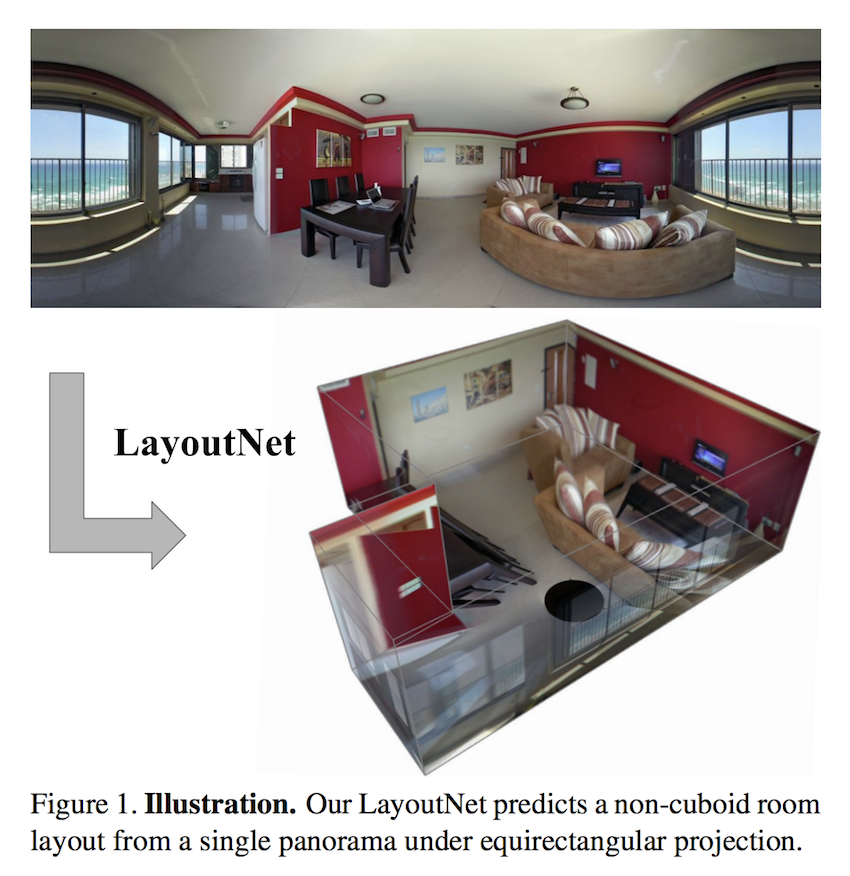
\includegraphics[width=\textwidth/2]{WPL/LON1.png}
\end{figure}
\begin{figure}
	\centering
	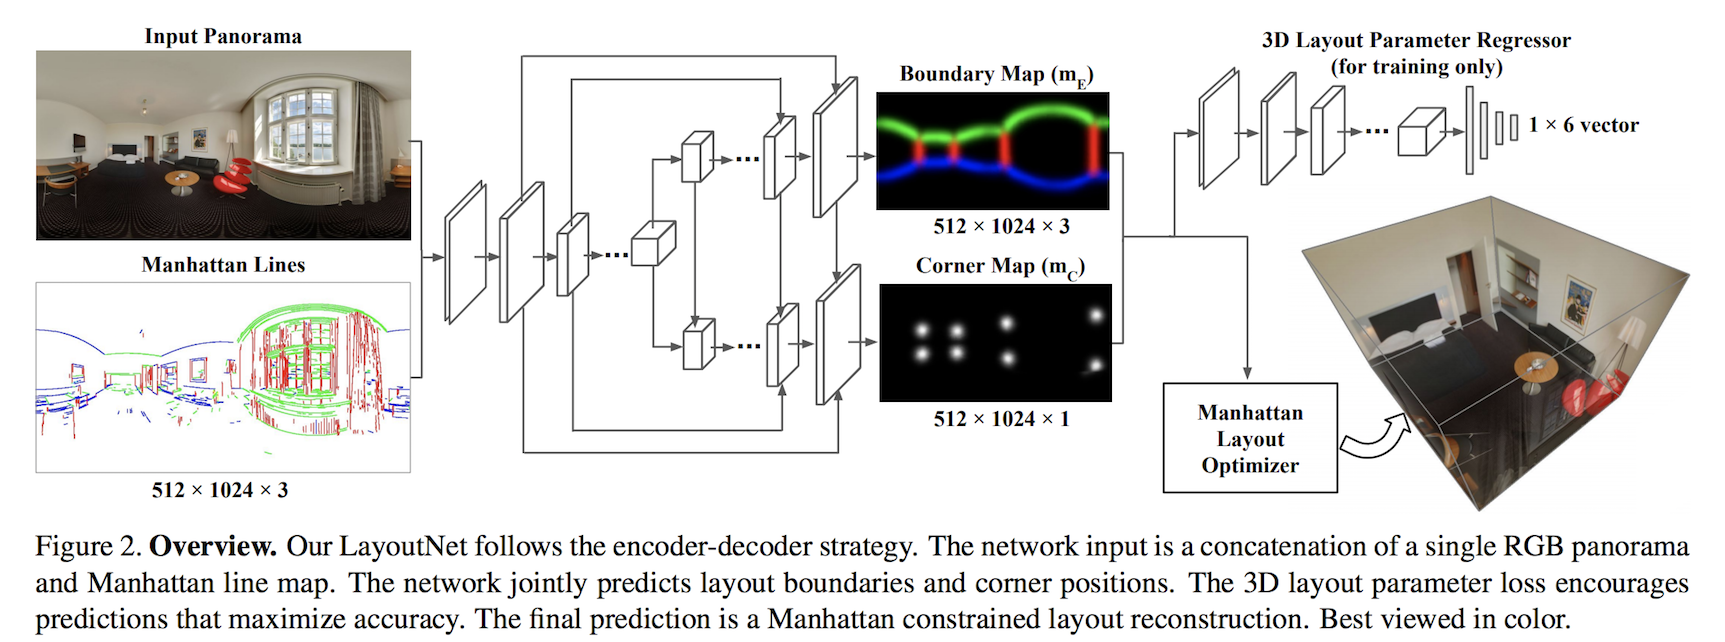
\includegraphics[width=\textwidth]{WPL/LON2.png}
\end{figure}

As we can observe in Figure 2, all the lines, edges and corners are detected for the input panorama image. These are the fed into the neural network which outputs the corner points. These points are then optimised by assuming a manhattan layout and the final layout of the room is obtained.

\subsubsection{Data Sets \& Code Bases}
({\em Within 50 words}) \\

Following open datasets are available for this application :

Hedau : \url{http://kobus.ca/research/data/CVPR\_13\_room/index.html}

LSUN : \url{http://lsun.cs.princeton.edu/2017/}

The code base for LayoutNet is available at 
\url{https://github.com/zouchuhang/LayoutNet}

%\noindent Identify open access code bases for the application. Compare if multiple sources are available.

\subsubsection{Conclusions}
({\em Within 50 words}) \\

The conversion of 2-D image into a 3-D layout has farfetching applications and would be very useful in mapping of buildings, roads efficiently. Though, the state-of-the-art technique is confined to manhattan layouts only, we hope that more techniques would be developed in the future to extend it to estimating layouts of complex, non-linear structures as well.

\newpage
\subsection{Application 2: Automatic enhancement of low-end camera photos}
%Use the same template as above.
\subsubsection{Introduction} 
({\em Within 100 words}) \\

The ever-increasing quality of camera sensors allows us to
photograph scenes with unprecedented detail and color. But
as one gets used to better quality standards, photos captured
just a few years ago with older hardware look dull and outdated.
Analogously, despite incredible advancement in quality
of images captured by mobile devices, compact sensors
and lenses make DSLR-quality unattainable for them, leaving
casual users with a constant dilemma of relying on their
lightweight mobile device or transporting a heavier-weight
camera around on a daily basis. However, the second option
may not even be possible for a number of other applications
such as autonomous driving or video surveillance systems,
where primitive cameras are usually employed. Hence, it is desired to
to have automated techniques which can enhance the images taken by low
end cameras. Previous works have explored using histogram equalization, photo
sharpening, contrast adjustment, etc for this use case. Here, we would be looking into WESPE (Weakly Supervised Photo Enhancer for Digital Cameras) which uses GANs to enhance low-end images and produce DSLR-quality images without requiring aligned original/enhanced photographs.

%\subsubsection{Motivation and Usage} ({\em Within 50 words)} 
\subsubsection{Sensors, Type \& Band of imaging}
({\em Within 50 words}) \\

The algorithm takes RGB images as input taken from mobile cameras or other low-end cameras.

\subsubsection{Algorithms / Processing} 
({\em Within 300 words})\\

%Details of the Algorithms and IP Components used at the major stages of the processing stack:

\begin{enumerate}
\item {\em \textbf{Style Transfer}}: The goal of style transfer is to apply the style of one image to
the (visual) content of another. Traditional texture/color/style
transfer techniques rely on an exemplar before/after
pair that defines the transfer to be applied. The
exemplar pair should contain visual content having a sufficient
level of analogy to the target image’s content which is
hard to find, and this hinders its automatic and mass usage.
More recently, neural style transfer alleviates this requirement. It builds on the assumption that the shallower
layers of a deep CNN classifier – or more precisely, their
correlations – characterize the style of an image, while the
deeper ones represent semantic content. A neural network is
then used to obtain an image matching the style of one input
and the content of another. Finally, generative adversarial
networks (GAN) append a discriminator CNN to a generator
network. The role of the former is to distinguish between
two domains of images: e.g., those having the style
of the target image and those produced by the generator. It
is jointly trained with the generator, whose role is in turn to
fool the discriminator by generating an image in the right domain,
i.e., the domain of images of correct style. WESPE exploits
this logic to force the produced images to be in the domain
of target high-quality photos.

\item {\em \textbf{Image Restoration}}: WESPE performs image quality enhancements through a list of its sub-tasks, like super-resolution, deblurring,
dehazing, denoising, colorization and image adjustment.
The goal of image super-resolution is to restore the original
image from its downscaled version using CNN. Losses based
on the activations of (a number of) VGG-layers and
GANs are more capable of recovering photorealistic results,
including high-frequency components, hence produce
state of the art results. In this work, both the
GAN architectures and VGG-based loss functions are incorporated.
Image colorization, which attempts to regress
the 3 RGB channels from images that were reduced to singlechannel
grayscale, strongly benefits from the GAN architecture. Image denoising, deblurring and dehazing, photographic style control and
transfer, as well as exposure correction are another
improvements and adjustments that are included in this
learned model.

\item {\em \textbf{Image to Image Enhancer}}: WESPE is build upon very recent advances in image-to-image
translation networks. Earlier approaches used a
general-purpose translator that takes advantage of GANs to
learn the loss function depending on the domain the target
image should be in. While it achieves promising results when
transferring between very different domains (e.g., aerial image
to street map), it lacks photorealism when generating
photos: results are often blurry and with strong checkerboard
artifacts. 
WESPE loosens this constraint by expressing the loss
in the space of input rather than output images, taking advantage
of a backward mapping CNN that transforms the output
back into the space of input images. However, the CNN architecture and loss functions
are based on different ideas: fully convolutional networks
and elaborated losses allows to achieve photorealistic
results, while eliminating typical artifacts (like blur and
checkerboard) and limitations of encoder-decoder networks.
Finally, it proposes an end-to-end enhancer
achieving photorealistic results for arbitrary-sized images
due to a composition of content, texture and color
losses. However, it is trained with a strong supervision requirement
for which a dataset of aligned ground truth image
pairs taken by different cameras was assembled (i.e., the
DPED dataset).

\end{enumerate}

\subsubsection{Example Illustration}
({\em Within 50 words}) \\

\begin{figure}
	\centering
	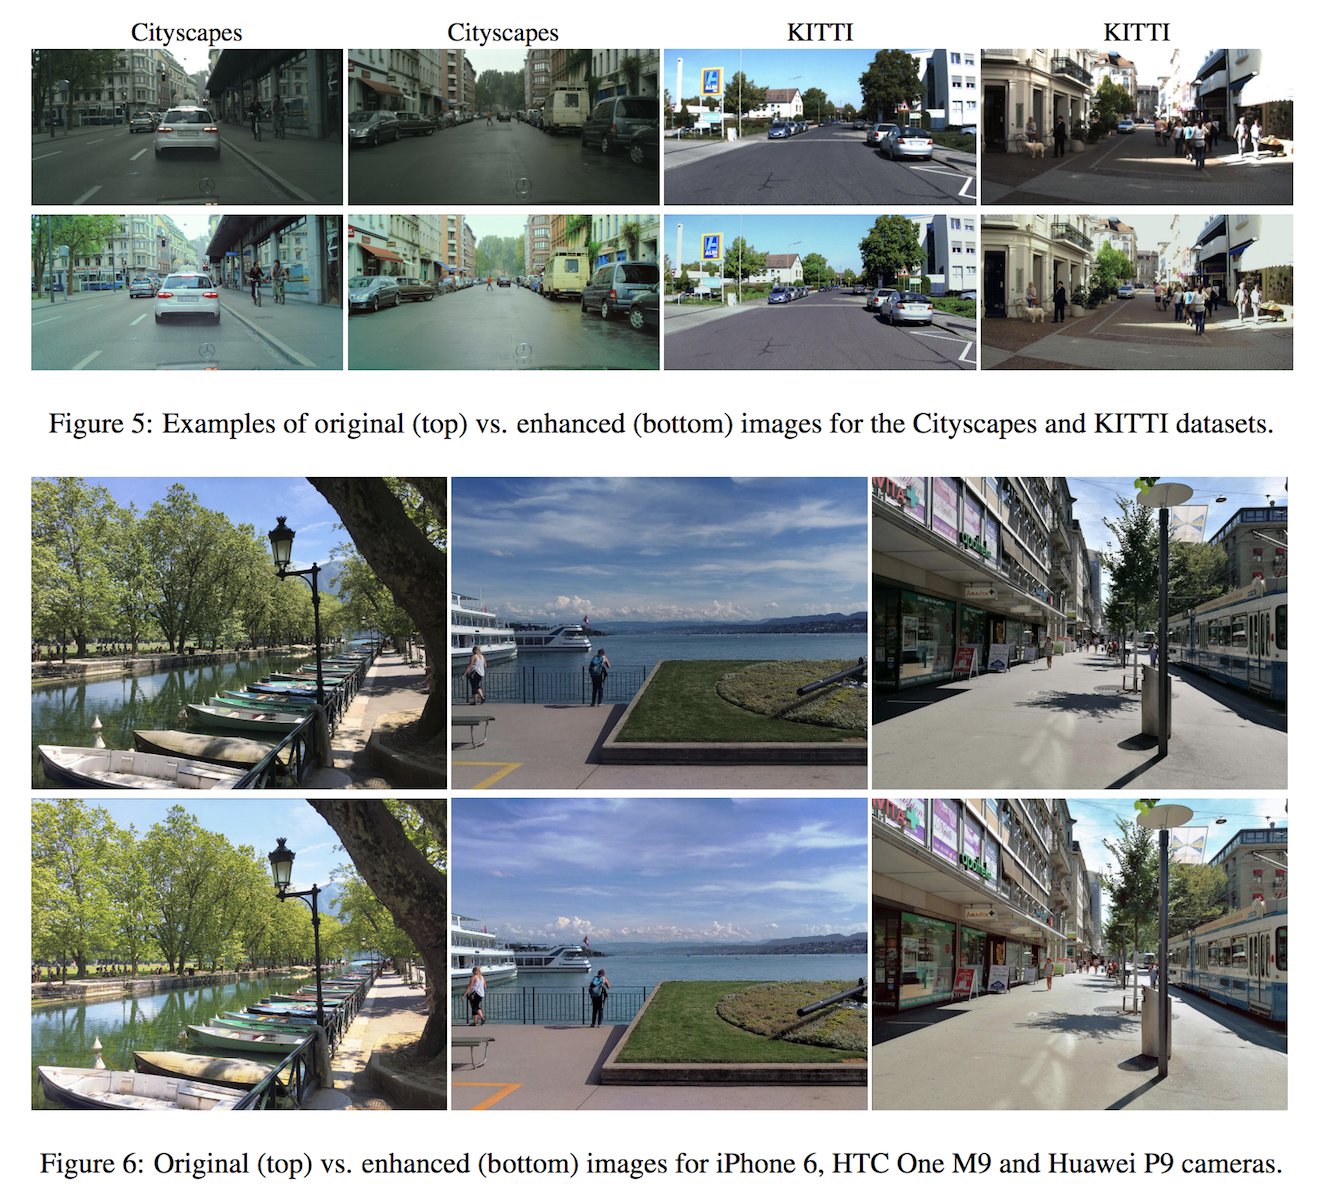
\includegraphics[width=\textwidth]{WPL/WESPE1.png}
\end{figure}

As depicted in the figure, the algorithm takes input an RGB image taken by a low-end camera and tries to enhance it to a DSLR-quality image

\subsubsection{Data Sets \& Code Bases}
({\em Within 50 words}) \\

Following open datasets are available for this application :

DPED : \url{http://people.ee.ethz.ch/~ihnatova/#dataset}

CityScapes : \url{https://www.cityscapes-dataset.com/}

Kitti : \url{http://www.cvlibs.net/datasets/kitti/}

The code base for WESPE is available at 
\url{https://github.com/aiff22/DPED}

\subsubsection{Conclusions}
({\em Within 50 words}) \\

Enhancing images to increase the quality is one of the most difficult tasks, and is usually done manually. This process has far-reaching secondary applications and is going to be more imperative in the future. WESPE is a breakthrough in this domain as it is weakly supervised and doesn't require much effort. In future, we hope that more such techniques would be developed to decrease the requirement of large annotated dataset.


\subsection{Application 3: 3-D reconstruction of a game using a monocular video}
%Use the same template as above.
\subsubsection{Introduction} 
({\em Within 100 words}) \\

Sports game analysis has been extensively
investigated from the perspectives of image processing,
computer vision, and computer graphics, both for
academic research and for industry applications. Understanding
a sports game involves several steps, from field
localization to player detection, tracking, segmentation, etc.
To do thorough analysis of the game, one needs to save as much information as possible from the game which is to save the complete game in 3-D.
One way to do this is to equip the
soccer field with many cameras, synchronize the cameras,
and then reconstruct the field and players in 3D using multiview
geometry techniques. The results
of multi-view methods are impressive, however the requirement
of physically instrumenting the field with many
synchronized cameras limits their generality. What if, instead,
we could reconstruct any soccer game just from a
single YouTube video? Here, we will be looking at the method proposed by the paper "Soccer On your Table Top" which does an end-to-end 3-D reconstruction of the game from just a monocular video of the game.

%\subsubsection{Motivation and Usage} ({\em Within 50 words)} 
\subsubsection{Sensors, Type \& Band of imaging}
({\em Within 50 words}) \\

The technique takes in a monocular video of a soccer game as input.

\subsubsection{Algorithms / Processing} 
({\em Within 300 words})\\

\begin{enumerate}
\item {\em \textbf{Camera Pose Estimation}}: The first step is to estimate the per-frame parameters of
the real game camera. Because soccer fields have specific
dimensions and structure according to the rules of FIFA, we
can estimate the camera parameters by aligning the image
with a synthetic planar field template. We set the world
origin to coincide with the center of the synthetic soccer
field which lies in the y = 0 plane. The most consistent features on the field of play are the
field lines (e.g., sidelines, penalty box around the goal).
Thus, we extract edge points E for each frame to localize
those features.

\item {\em \textbf{Player Detection and Tracking}}: The first step of the video analysis is to detect the players
in every frame. We start with a set of bounding boxes.
Next, we refine the initial bounding boxes based on pose information
using the detected keypoints/skeletons.
We observed that the estimated poses can better separate
the players than just the bounding boxes, and the pose keypoints
can be effectively used for tracking the players across
frames.
Finally, we generate tracks over the sequence based on
the refined bounding boxes.
Every track has a starting and
ending location in the video sequence. The distance between
two tracks A and B is defined as the 2D Euclidean
distance between the ending location of track A and starting
location of track B, assuming track B starts at a later
frame than track A and their frame difference is smaller
than a threshold (detailed parameters are described in supplementary
material). We follow a greedy merging strategy.
We start by considering all detected neck keypoints
(we found this keypoint to be the most reliable to associate
with a particular player) from all frames as separate tracks
and we calculate their pairwise distances. Two tracks are
merged if their distance is below a threshold, and we continue
until there are no tracks to merge. This step associates
every player with a set of bounding boxes and poses across
frames. This information is essential for the later processing
of the players, namely the temporal segmentation, depth estimation
and better placement in 3D.
Fig. 2 shows the steps
of detection, pose estimation, and tracking.

\item {\em \textbf{Temporal Instance Segmentation}}: For every tracked player we need to estimate its segmentation
mask to be used in the depth estimation network. A
straightforward approach is to apply at each frame a person
segmentation method, refined with a dense CRF as
we did for training. This can work well for the unoccluded
players, but in the case of overlap, the network estimates are
confused. Although there are training samples with occlusion,
their number is not sufficient for the network to estimate
the depth of one player (e.g. the one closer to the center)
and assign the rest to the background. For this reason,
we “help” the depth estimation network by providing a segmentation
mask where the tracked player is the foreground
and the field, stadium and other players are background (this
is similar to the instance segmentation problem, but
in a 1-vs-all scenario).

\item {\em \textbf{Mesh Generation}}: The foreground mask from the previous step, together
with the original cropped image are fed to the depth estimation network. The output of the network is per-pixel, quantized
signed distances between the player’s surface and a
virtual plane w.r.t. the camera. To obtain a metric depth
map we first lift the bounding box of the player into 3D,
creating a billboard (we assume that the bottom pixel of the
player lies on the ground). We then apply the distance offsets
output by the network to the 3D billboard to obtain the
desired depth map.
The depth map is then unprojected to world coordinates
using the camera parameters, generating the player’s pointcloud
in 3D. Each pixel corresponds to a 3D point and we
use pixel connectivity to establish faces. We texture-map
the mesh with the input image. Depending on the application,
the mesh can be further simplified with mesh decimation
to reduce the file size for deployment in an AR device.

\item {\em \textbf{Trajectories in 3D}}: Due to imprecise camera calibration and bounding box
localization, the 3D placement of players can “jitter” from
frame to frame. To address this problem, we smooth the 3D
trajectories of the players. In particular, once we estimate
the player’s position in the 3D field, we calculate the center
of the mesh (mean of the player’s vertices) and solve for its
optimized 3D trajectory.

\end{enumerate}

\subsubsection{Example Illustration}
({\em Within 50 words}) \\

\begin{figure}
	\centering
	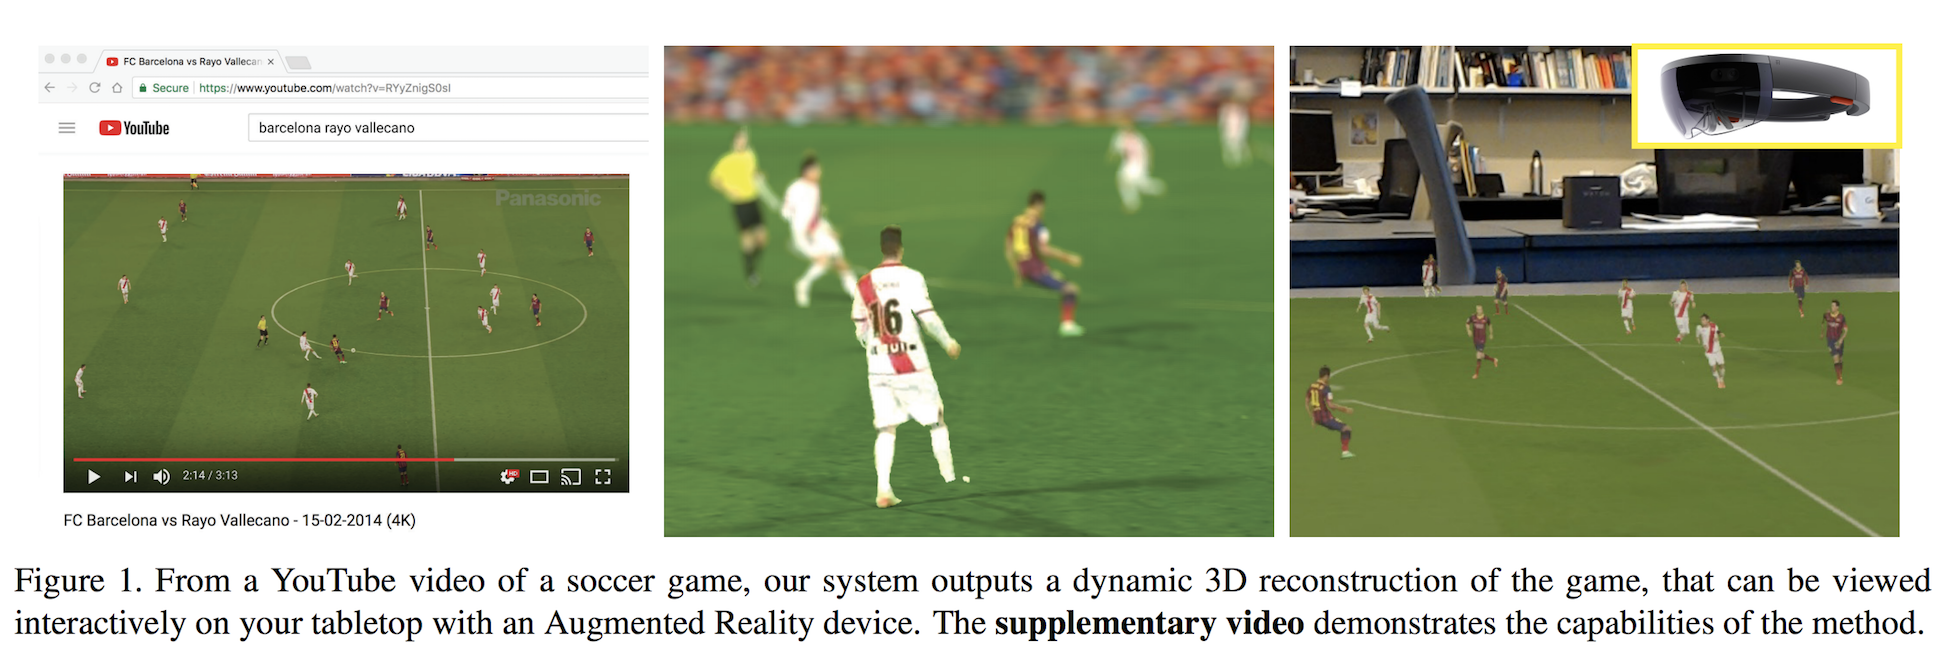
\includegraphics[width=\textwidth]{WPL/SOYTT1.png}
\end{figure}
\begin{figure}
	\centering
	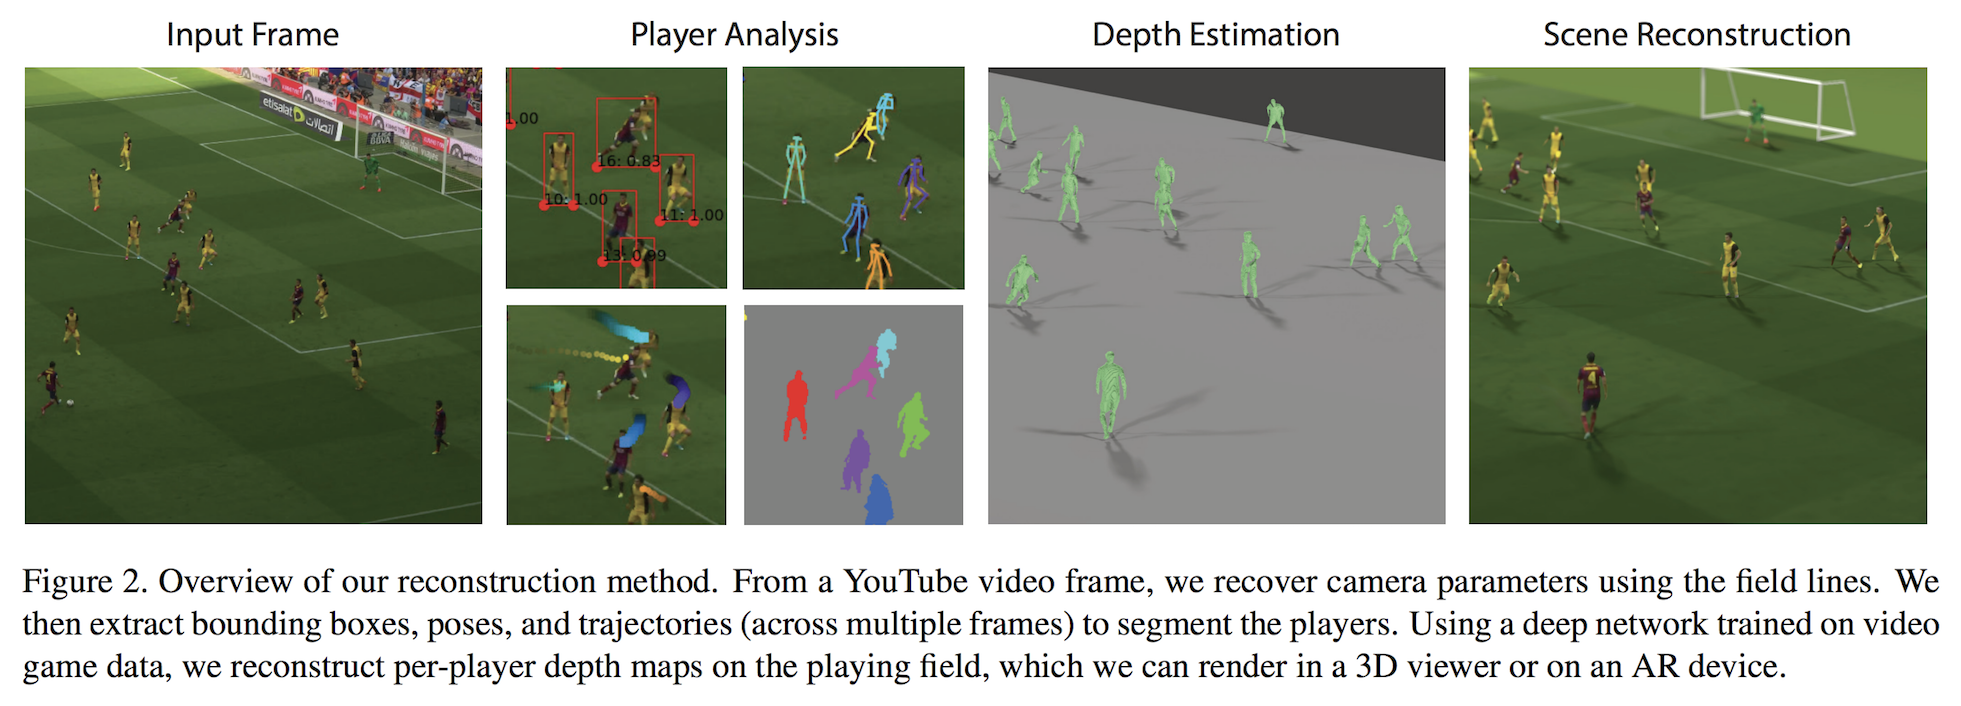
\includegraphics[width=\textwidth]{WPL/SOYTT2.png}
\end{figure}

As we can see in the figure, for each frame, first players are identified, there trajecteries are calculated using the sequence of frames, depth estimation is performed and then the scene is reonstructed.

\subsubsection{Data Sets \& Code Bases}
({\em Within 50 words}) \\

For training data, images and their corresponding depths were extracted while playing FIFA game.

The code base for "Soccer On your Tabletop" is available at 
\url{https://github.com/krematas/soccerontable}

\subsubsection{Conclusions}
({\em Within 50 words}) \\

Soccer On your Table Top is a state-of-the-art technique for 3-D reconstruction of football games from a simple monocular video of it. The technique might be extended to other field games as well like hockey, rugby, etc. In future, we hope that such techniques would develop for other games as well where the background is not uniform like a field. It would be interesting to explore its use in other domains such as 3-D reconstruction of security footage, etc.

\section{Your new Idea}
({\em Within 100 words})\\

As we see that a lot of professors are unhappy with students bunking their classes. But, the more bothersome thing for a professor is that they put proxy too. Now, its not always efficient for a professor to take attendance in the class as it takes time off the lecture hour and if its a big class then forget about it. Now, the best solution might be to just remove the attendance itself but at the end of the day, everyone needs to adhere to the institute policy which doesn't allow free attendance. Hence, to save the time from the lecture hour or the efforts of the TAs to move around with the attendance sheet, my new idea is to detect proxy signatures from a scanned image of an attendance sheet automatically. 
%If its a blank sheet then the people whose proxies were put and those who put it would have their signatures close by. And if its a printed sheet then they might have been signed with the same pen. I think it should be feasible by identifying the colour of the pens, the slantness of the handwriting and the pressure with which the signatures were put. So, though the signatures would have been put in a different handwriting they may still collide with respect to above details. The algorithm should not reject any false negatives. This program may also keep track for changes in signatures of a person over the days as the original and the proxy would definitely not be the same.

\section{References}
\begin{enumerate}
    \item {LayoutNet}: \url{https://arxiv.org/abs/1803.08999}
    \item {WESPE}: \url{https://arxiv.org/pdf/1709.01118.pdf}
    \item {Soccer on your Table Top}: \url{https://arxiv.org/abs/1806.00890}
\end{enumerate}
\end{document}